\documentclass[12pt]{article}
\usepackage[utf8]{inputenc}

\usepackage{hyperref}
\usepackage{wrapfig}
\usepackage{amsmath}
\usepackage{minted}
\usepackage{color}
\usepackage{svg}
\usepackage{graphicx}
\usepackage{fancyhdr}
\usepackage{natbib}

\bibliographystyle{humannat}

\graphicspath{ {./images/} }
\setlength{\tabcolsep}{10pt}
\setlength{\headheight}{15pt}

\providecommand{\shortcite}[1]{\cite{#1}}

\title{A visualiser for $\lambda$-terms as rooted 3-valent maps}
\author{George Kaye}
\date{March 2019}

\makeatletter

\pagestyle{fancy}
\fancyhf{}
\fancyhead[R]{\textsl{\rightmark}}
\fancyfoot[C]{\thepage}

\renewcommand{\footrulewidth}{0.5pt}

\begin{document}

\input{titlepage.tex}

\tableofcontents

\newpage

\section{Abstract}
\label{sec:abstract}
Todo

\newpage

\section{Acknowledgements}
\label{sec:acks}
Todo


\newpage

\section{Introduction}
\label{sec:intro}

This report details the development of a set of tools to aid in the research of the topological properties of $\lambda$-terms when they are represented as rooted maps.

\subsection{\texorpdfstring{$\lambda$}{lambda}-term visualiser}

Drawing $\lambda$-terms maps by hand can be quite time-consuming, especially for large terms. The first tool can generate maps for $\lambda$-terms from user input, in addition to providing interesting properties such as crossings. By visualising the $\lambda$-terms it can become much easier to understand the structure of more complex structures implemented in the $\lambda$-calculus (such as pairs).

The visualiser also has functionality relating to the normalisation of terms. The $\beta$-redexes contained within the term are listed, and by clicking on these the user can reduce the term to its normal form (if one exists). A normalisation graph can also be generated, which can also be interesting to examine.

\subsection{\texorpdfstring{$\lambda$}{lambda}-term gallery}
When studying properties of $\lambda$-terms, it can be useful to generate terms and look for interesting properties shared between terms and their maps. However it can be tricky to come up with terms with certain properties (such as terms containing a certain amount of subterms) on the fly. The $\lambda$-term gallery can generate all terms of a certain size and free variables, with the ability to filter based on properties such as crossings or $\beta$-redexes. This makes testing conjectures a much easier process.

From the gallery, the user can inspect the generated terms using the visualiser, with the same functionality present as detailed above.

\begin{figure}
    \centering
    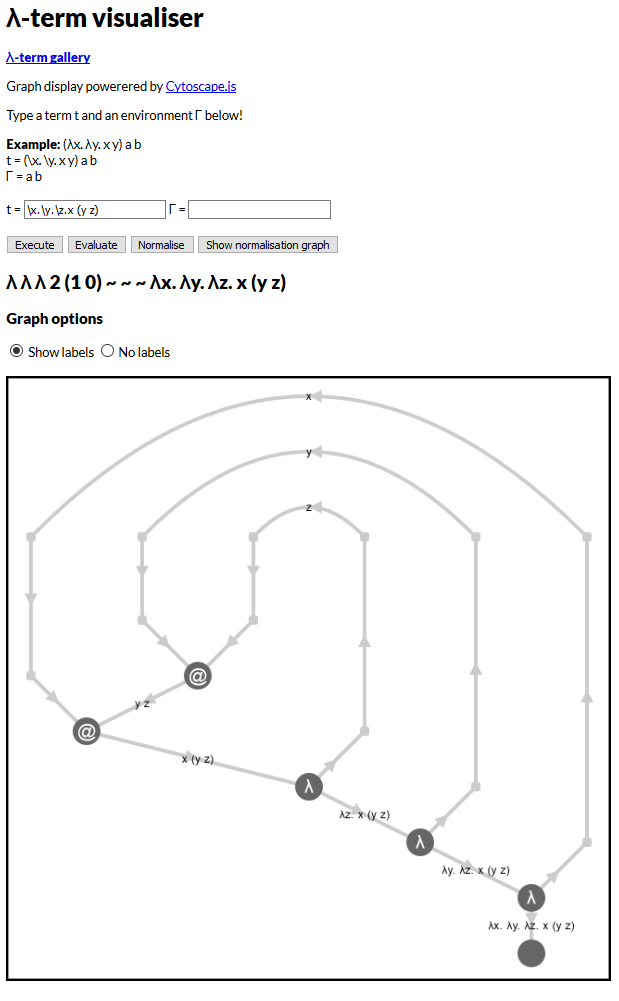
\includegraphics[scale=0.3]{visualiser}
    \caption{The $\lambda$-term visualiser, displaying the map for the term $\lambda x. \lambda y. \lambda z. x \, (y \, z)$, along with some statistics on the right.}
    \label{fig:visualiser}
\end{figure}

\begin{figure}
    \centering
    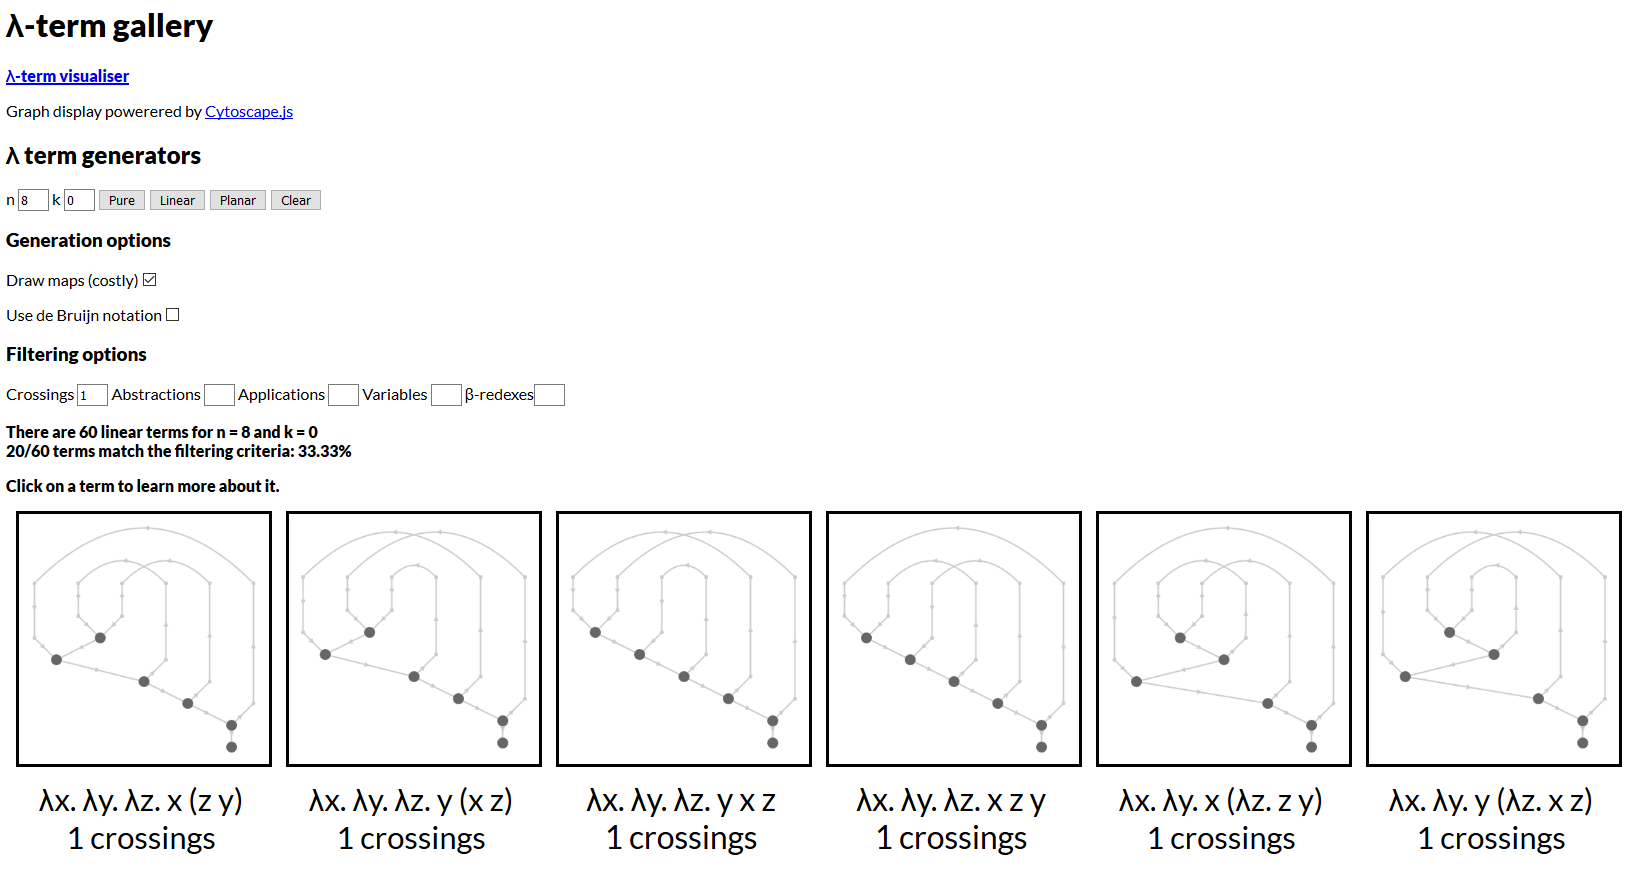
\includegraphics[scale=0.3]{gallery}
    \caption{The $\lambda$-term gallery, displaying all closed linear terms of size 5.}
    \label{fig:gallery}
\end{figure}

\newpage

\section{Background}
\label{sec:background}

\subsection{The \texorpdfstring{$\lambda$}{lambda}-calculus}
The $\lambda$-calculus is a model of computation where programs are represented by variable abstraction and function application. It is the basis of all functional programming languages. This section will cover some concepts and terminology that will be used in the remainder of the report.

\subsubsection{Definitions}
\label{sec:defs}

The simplest terms in the $\lambda$-calculus ($\lambda$-terms) are just \textbf{variables} ($x, y, z, ...$). More complex terms can be created using the operations of \textbf{abstraction} ($\lambda x. T$) and \textbf{application} $(T_1 T_2)$. For clearer notation, applications are left-associative and abstractions extend as far to the right as possible:
%
\begin{align*}
    x \, y \, z &\equiv (x \, y) \, z \\
    \lambda x. x \, \lambda y. y &\equiv (\lambda x. x \, (\lambda y. y))
\end{align*}
%
Variables in the $\lambda$-calculus can be \textbf{bound} or \textbf{free}. A variable is bound if it is inside the scope of a corresponding $\lambda$-abstraction (it is a local variable), or free otherwise. In $\lambda x. x \, y$, the $x$ is bound but the $y$ is free. A $\lambda$-term with no free variables is called a \textbf{closed term}. Two $\lambda$-terms are said to be \textbf{$\alpha$-equivalent} if the only difference between them is the names of their bound variables -- for example, $\lambda x. x$ and $\lambda y. y$ are $\alpha$-equivalent. The process of renaming bound variables is known as \textbf{$\alpha$-conversion}:
%
$$\lambda x. T \to_\alpha \lambda y. T[x \mapsto y]$$
%
To avoid ambiguity between $\alpha$-equivalent terms, we can use \textbf{de Bruijn notation}. Rather than using explicit variable names, each variable is instead represented by how 'far away' the corresponding abstraction is. For example, $\lambda x. \lambda y. \lambda z. x \, y \, z$ can be written as $\lambda\lambda\lambda \, 2 \, 1 \, 0$. This eliminates the need for $\alpha$-conversion and makes it far more efficient to determine equality of $\lambda$-terms.

$\lambda$-terms contain a number of \textbf{subterms}, defined as:
%
\begin{align*}
    subterms(x) &= 1 \\
    subterms(\lambda x. T) &= 1 + subterms(T) \\
    subterms(T_1 T_2) &= 1 + subterms(T_1) \, + \, subterms(T_2)
\end{align*}

\subsubsection{\texorpdfstring{$\beta$}{Beta}-reduction}

Program execution in the $\lambda$-calculus is performed through \textbf{$\beta$-reduction} -- applying functions to their arguments. A term of the form $(\lambda x. T_1) \, T_2$ is called a \textbf{$\beta$-redex} and can be $\beta$-reduced as follows:
%
$$(\lambda x. T) \, u \to_\beta T[x \mapsto u]$$
%
Repeatedly performing $\beta$-reduction on a term until it contains no $\beta$-redexes is known as \textbf{normalisation}. A term with no $\beta$-redexes is in its \textbf{normal form}. All $\lambda$-terms have a unique normal form but for some terms this normal form is not computable. While there may be multiple redexes to choose from in a given $\lambda$-term, the order of reductions does not matter and the same normal form will be reached if it is computable -- this is known as the \textbf{Church-Rosser theorem}. The process of normalisation can be represented by \textbf{normalisation graphs}, which show the various paths between a $\lambda$-term and its normal form. An example of normalisation graphs can be seen in Figure \ref{fig:normgraphs}.

\begin{figure}
    \centering
    \includegraphics{reduction}
    \caption{An example of two normalisation graphs, showing the steps of reduction taken for the terms $\lambda x. (\lambda y \, x) (\lambda z. z)$ and $\lambda x. (\lambda y. y) ((\lambda z. z) \, x)$ to reach their normal forms. Note that the diverging paths in the right example still lead to the same normal form, as stated by the Church-Rosser theorem.}
    \label{fig:normgraphs}
\end{figure}

\subsubsection{Fragments of the \texorpdfstring{$\lambda$}{lambda}-calculus}
The \textbf{pure $\lambda$-calculus} contains all terms formed from combining variables, abstractions and applications. However we can restrict ourselves to smaller \textbf{fragments} of the $\lambda$-calculus. The \textbf{linear $\lambda$-calculus} is a subset of the pure $\lambda$-calculus containing terms in which variables are used exactly once, and the \textbf{planar $\lambda$-calculus} is a subset of the linear $\lambda$-calculus in which variables are used in the order they are abstracted in. Linear and planar $\lambda$-terms have special properties relating to maps, which will be covered in the next section.

\begin{table}
    \centering
    \begin{tabular}{|c|c|c|c|}
        \hline
        \textbf{Term} & \textbf{Pure} & \textbf{Linear} & \textbf{Planar} \\
        \hline
        $\lambda x. x$ & Yes & Yes & Yes \\
        \hline
        $\lambda x. (\lambda y. y) \, x$ & Yes & Yes & Yes \\
        \hline
        $\lambda x.\lambda y. x \, y$ & Yes & Yes & Yes \\
        \hline
        $\lambda x. \lambda y. y \, x$ & Yes & Yes & No \\
        \hline
        $\lambda x. x \, x$ & Yes & No & No \\
        \hline
    \end{tabular}
    \caption{Examples of terms in various fragments of the $\lambda$-calculus.}
    \label{tab:fragments}
\end{table}

\subsection{Graphs and maps}

\begin{figure}
    \centering
    \includesvg{maps}
    \caption{These two diagrams represent the same graph but two distinct maps (the ordering of edges around the point on the circle is changed). Adapted from Lando, Zvonkin {\cite{graphs}}}
    \label{fig:maps}
\end{figure}

In graph theory, a \textbf{graph} is a set of nodes and edges that link pairs of nodes. When these graphs are \textbf{embedded} onto a surface they are called \textbf{maps}. Unlike graphs, the order of edges around a node is important for maps, and the same graph can be represented as many different maps (an example is shown in Figure \ref{fig:maps}). A map has a \textbf{genus} which is how many 'holes' the surface it is embedded into has. \textbf{Planar maps} are maps with no crossings of edges -- they have a genus of 0. 

In this project we are particularly interested with \textbf{rooted 3-valent maps}. The \textbf{valency} of a node is how many edges connect to it - maps where all of the nodes have a valency of 3 are called \textbf{3-valent}. We can make a \textbf{rooted map} by adding a 'special' node (the \textbf{root}) that connects to the map at one point, as shown in Figure \ref{fig:trivalentrooted}.

\begin{figure}
    \centering
    \includegraphics[scale=0.3]{torus}
    \caption{An example of how a graph with crossings can be embedded onto a torus. From \shortcite{zeil4ct}.}
    \label{fig:torus}
\end{figure}

\begin{figure}
    \centering
    \includesvg[scale=0.5]{trivalentrooted}
    \caption{A 3-valent map, and the same map but rooted (root indicated by the white node)}
    \label{fig:trivalentrooted}
\end{figure}

We can represent $\lambda$-terms as maps. Abstractions and applications are represented as nodes, as shown in Figure \ref{fig:absapp}. With the addition of a root to represent the start of the term, these nodes can be combined to create a rooted map, as shown in Figure \ref{fig:trivalentrooted}.

Viewing these $\lambda$-term maps can be interesting for many reasons. We can tell which terms are linear since their corresponding maps are 3-valent -- abstracted variables are only used once. Planar terms correspond to planar graphs with no crossings.

\begin{figure}
    \centering
    \includegraphics[scale=0.7]{absapp}
    \caption{An abstraction and an application, represented as nodes of a map.}
    \label{fig:absapp}
\end{figure}

\begin{figure}
    \centering
    \includegraphics[scale=0.8]{lambdatermandgraph}
    \caption{A representation of the term $\lambda x. \lambda y. \lambda z. x \, (y \, z)$ as a rooted 3-valent map, without and with node labels. From \protect\cite{zeiljfp}.}
    \label{fig:lambdatermandgrapht}
\end{figure}

\newpage

\section{Features}


\section{Design}
\label{sec:design}

The two tools 

\subsection{\texorpdfstring{$\lambda$}{Lambda}-term visualiser}


\subsection{\texorpdfstring{$\lambda$}{Lambda}-term gallery}



\newpage

\section{Implementation}
\label{sec:implementation}

This section will cover the implementation of the tools, and issues that rose.

\subsection{Language}
To implement the tools, I decided to use \texttt{Javascript}. This was so the tools could be distributed as 'web apps' and hosted on a website rather than having to be downloaded and relying on any dependencies.

\subsection{Implementing the \texorpdfstring{$\lambda$}{lambda}-calculus in \texttt{Javascript}}
The first part of developing the project was to implement the $\lambda$-calculus in \texttt{Javascript}, as a basis for the rest of the project to build on. The implementation partially based on the \texttt{ML} examples developed by \cite{pierce}. Variables are stored as de Bruijn indices -- this means that it is trivial to tell if terms are identical without having to perform $\alpha$-conversion. Abstractions and applications are constructed as combinations of subterms. Functionality was added later in the project so that terms can be associated with an \textbf{alias} to save time when writing out large expressions (for example, the alias \texttt{id} for the identity function $\lambda x. x$).

Since terms often contain free variables, a class to represent the context of a term was also created. This was effectively a wrapper for an array that contained the labels of terms currently in the context, with some extra methods to make manipulating it easier, such as determining a label from a given de Bruijn index. 

Printing the $\lambda$-terms proved to be more nuanced than expected. While the de Bruijn representation of a term is constant and easy to print, it is not very readable (especially in large terms) -- traditional labelled terms are much more intuitive. Originally variables stored a 'label' that could be printed instead of the index, but this proved to be quite buggy and often variables and their corresponding abstractions would display different labels (e.g. after $\alpha$-conversion). To fix this, labels were restricted to just abstractions, and when printing these labels would be added to a context. When the variables were to be printed, the index of the term would be looked up in the context and the appropriate label retrieved. This would ensure consistency (and subsequently correctness) throughout the term. 

When implementing the normalisation functionality, it became apparent that some sort of $\alpha$-conversion would still need to be implemented to avoid clashes of variables in the printed labels. A function was implemented to generate a 'canonical' set of labels, to ensure that each variable name was only used once in the term. For example, the term $(\lambda d. (\lambda h. h \, d) \, h) \, g$ with free variables $h$ and $g$ would be $\alpha$-converted to $\lambda x. (\lambda y. y \, x) \, a) \, b$. This would also be used when generating normalisation graphs later on -- redexes that led to $\alpha$-equivalent terms would have a consistent set of labels rather than juggling many different representations.

\subsection{Parsing terms from user input}
Initially the parser would iterate through the user input one character at a time, making note of 'special' characters (e.g. a backslash to represent a $\lambda$-abstraction, or an opening bracket to indicate the start of a subterm). It would then create the $\lambda$-term objects as it went from left to right. However the original parsing algorithm grew quite confusing, as it had to keep track of many different states (e.g. if an abstraction was in progress), and in practice elements could be more than one character long (such as longer variable names).

To make the process more intuitive, parsing was split into two distinct parts: an initial tokenising phase where the input would be split into the different tokens (e.g. $\lambda var. (\lambda y. y) \, var \implies$ \texttt{[\textbackslash,var,(,\textbackslash,y,),var)]}), and the parsing phase where these tokens would be formed into actual $\lambda$-terms. The benefit of tokenising first is that syntax errors (such as mismatched brackets or missing abstraction variables) are caught first, and the parser can iterate over tokens without having to worry about malformed terms. This also means that the parsing process is consistent even if variable names are longer than one character, as the labels can be stored as one token. 

This means that the 'special characters' the parser needs to check for are \texttt{(} and \texttt{)} for subterms, and \texttt{\textbackslash} for abstractions. Everything else is a variable, and adjacent tokens/subterms represent applications. To extend the parser to handle aliases, all that had to be added was to check tokens against the list of existing aliases, and use the corresponding function body if one existed.

\subsection{Drawing the terms}
Developing a suitable way of drawing the $\lambda$-term maps was the first major problem in the project. Drawing correct maps by hand is quite intuitive as one can place nodes and their edges 'on the fly' so that they do not cross over. However implementing an algorithm for a computer to generate these maps is significantly more difficult.

\subsection{\texorpdfstring{$\lambda$}{Lambda}-term 'portraits'}

\subsection{Enumeration and generation functions}

\subsection{The gallery}

\subsection{Normalisation}

\begin{figure}
    \begin{minted}[frame=lines]{js}
    class LambdaVariable { 
        constructor(index, alias); 
    }
    class LambdaAbstraction { 
        constructor(t, label, alias); 
    }
    class LambdaApplication { 
        constructor(t1, t2, alias); 
    }
    
    /* representing swap = \x.\y.y x */
    const var1 = new LambdaVariable(0);     
    const var2 = new LambdaVariable(1);      
    const app = new LambdaApplication(var1, var2);  
    const abs1 = new LambdaAbstraction(app, 'y');    
    const abs2 = new LambdaAbstraction(abs, 'x', 'swap');   
    
    \end{minted}
    \caption{The constructors of the three types of $\lambda$-terms, implemented in \texttt{Javascript}, as well as an example of how the function $swap = \lambda x. \lambda y. y x$ would be implemented.}
    \label{fig:implementation}
\end{figure}
\newpage

\section{Conclusion}
\label{sec:conclusion}
Todo

\newpage

\bibliography{refs}

\end{document}
